\documentclass[11pt,reqno]{amsart}
\oddsidemargin = 0cm \evensidemargin = 0cm \textwidth = 16cm

\usepackage{amssymb,amsfonts,amscd,amsbsy}
\usepackage[mathscr]{eucal}
\usepackage{url}
\usepackage[ruled,vlined]{algorithm2e}

\usepackage{amsmath}
\usepackage{listings}
\lstset{numbers=left, numberstyle=\small, stepnumber=1, numbersep=5pt}
\usepackage{tikz}
\usetikzlibrary{arrows}
\usetikzlibrary{positioning}

\newtheorem{thm}{Theorem}[section]
\newtheorem{claim}[thm]{Claim}
\newtheorem{lem}[thm]{Lemma}
\newtheorem{prop}[thm]{Proposition}
\newtheorem{cor}[thm]{Corollary}
\newtheorem{oper}[thm]{ADT Operation}
\usepackage{pgfkeys}
\usepackage{hyperref}
\theoremstyle{definition}
\newtheorem{definition}{Definition}
\newtheorem{remark}[thm]{Remark}
\newtheorem{example}[thm]{Example}
\numberwithin{equation}{section}


\tikzstyle{vertex}=[circle,fill=black!25,minimum size=20pt,inner sep=0pt]
\tikzstyle{selected vertex} = [vertex, fill=red!24]
\tikzstyle{edge} = [draw,thick,-]
\tikzstyle{weight} = [font=\small]
\tikzstyle{selected edge} = [draw,line width=5pt,-,red!50]
\tikzstyle{ignored edge} = [draw,line width=5pt,-,black!20]

\begin{document}
	
	\title[COMP20230 - Graphs - Lecture 16]{COMP20230 - Graphs (1) - Lecture 16}
	
	\author{Adam Ryan and Shivam Bhatia}
	
	\address{School of Computer Science, University College Dublin, Belfield, Dublin 4, Ireland}
	
	\email{adam.ryan@ucdconnect.ie}
	
	\email{shivam.bhatia@ucdconnect.ie}
	
	\keywords{Graph Theory, COMP20230, Lecture Notes}
	
	\date{\today}
	
	\begin{abstract}\label{abstract}
		As part of the COMP20230 module, students are required to compile lectures notes on a topic which they have chosen. These lecture notes are worth $20\%$ of the student's grade in the module. \\
		\\
		In this paper, the authors compile lecture notes on the Graph ADT covered in Lecture 16, examining the definition of a graph, operations associated with the Graph ADT, matrix representations of a graph, and examine the DFS and BFS algorithms.
	\end{abstract}
	
	\maketitle
	
	\pagebreak
	\tableofcontents
	\pagebreak
	
	
	\section{Introduction}\label{intro}
	\noindent In this section, we introduce the reader to the concept of graphs, and provide a number of relatively informal definitions surrounding what a graph is. We motivate these definitions by highlighting a few example graphs which cover various types of graphs that are captured by the Graph ADT. In later sections, we will motivate these definitions with historical context, and delve more firmly into the Graph ADT specifically rather than viewing it from the context of Graph Theory.
	
	\begin{definition}\label{graph}
		A graph $G=(V,E)$ is comprised of a set of vertices (also referred to as nodes) (V) and pairs of vertices $((u,v) : u,v \in V)$  called edges (E). Implicitly, non-connected components are allowed within Graphs. This is visually represented by a series of points connected with straight lines (the edges) as in figure \ref{fig:K5}
	\end{definition}
		
	\begin{remark}
		A common shorthand notation for refering to an edge $(u,v)$ is $uv$ which denotes that the vertices $u$ and $v$ are connected.
	\end{remark}

	\begin{definition}\label{degree}
		For a graph $G=(V,E)$ and $v \in V$, we say the degree of v denoted $d(v)$ is the number of edges connected to that vertex. The degree sequence of a graph is the set $\{d(v): v\in V\}$.\\
	\end{definition}

	\begin{definition}\label{degree}
		The order of a graph is $|V|$ (i.e. the number of vertices). 
	\end{definition}

	\begin{definition}\label{degree}
		The size of a graph is $|E|$ (i.e. the number of edges).
	\end{definition}

	\begin{definition}
		If the set E consists of ordered pairs of vertices, then G is referred to as a digraph or directed graph. In a digraph, edges are represented with an arrow indicating the direction that the edge can be traversed.
	\end{definition}

	\begin{definition}
		If the set E is a multiset (i.e. the same two vertices can be joined by more than one edge) then G is referred to as a multigraph.
	\end{definition}
		
	\begin{definition}
		If the set E allows a pair of vertices such that each vertex is identical, and E is a multiset, then G is referred to as a pseudograph.
	\end{definition}

\begin{definition}
	A cycle in a graph is a series of edges $(e_1, e_2, ... e_n)$ with a vertex sequence $(v_1,v_2,...v_m)$ where $v_1=v_m$. More informally, a cycle in a simple graph is a collection of edges that start and end at the same vertex where no edge is repeated. An Eulerian cycle is a cycle in which $(e_1,e_2,...e_n)=E$, and a Hamiltonian cycle is a cycle where all vertices are used exactly once.
\end{definition}
		
	\begin{definition}
		A graph which contains no cycles is called a forest.
	\end{definition}

\begin{remark}
	Note that some authors have alternative definitions of trees and forests such that a tree is an acyclic connected graph, while a forest is a union of trees such that, for a forest G, $K(G)>1$. This definition is not equivalent to the above. This is easily shown by noting that using the definition above, all forests are trees (by definition) whereas with the alternative definition trees are by definition not forests. For the remainder of this, we will use the definition above rather than this as it's commonly used for combinatorial arguments (see \href{https://people.math.umass.edu/~raymond/math455/ws13-solutions.pdf}{University of Massachusetss Q4's inclusion of Trees with K(G)=1 as an example}).
\end{remark}

\begin{definition}
		A forest which is connected is called a Tree (i.e. a Tree is a connected graph without cycles).
\end{definition}

\begin{definition}
	A weighted graph is a graph where each edge is assigned a weight.
\end{definition}
	
\begin{definition}\label{GADT}
		Within the Graph ADT, we consider both digraphs and pseudographs, and will henceforth refer to these simply as 'Graphs'. To be explicit, the Graph ADT is a data type which includes graphs which can multiple edges between the same points, where edges can be present linking nodes to themselves, weighted graphs, and also graphs where edges can only be traversed in certain directions. The Graph ADT is similar to a Tree ADT, however unlike Trees, Graphs are allowed to contain cycles and disconnected components.
	\end{definition}
	
	\noindent In the above, we have quickly given a number of definitions concerning graphs, however to put these in context a number of graphs are presented below as examples for the reader to contextualise graphs, and the various types of graphs defined previously. 
	\begin{example}
		In figure \ref{fig:K5}, we have a sample graph $K_5$. In this graph we have:\\ \\$V=\{v_1,v_2,v_3,v_4,v_5\}$
		\\
		\\$E=\{(v_1,v_2), (v_1,v_3), (v_1,v_4), (v_1,v_5) ,(v_2,v_3), (v_2,v_4), (v_2,v_5),(v_3,v_4), (v_3,v_5), (v_4,v_5)\}$\\
		\\
		In this graph, we see that each of the five vertices are connected to every other vertex in the graph, and can identify a number of cycles are present, such as  $v_1 \rightarrow v_4 \rightarrow v_5 \rightarrow v_1$.\\
		\\
		The order of this graph is $5$, while the size of this graph is $10$, and each vertex has degree 4.
		\begin{figure}[h!]
			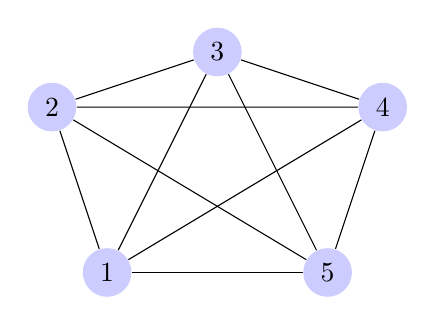
\begin{tikzpicture}
				[scale=.35,auto=left,every node/.style={circle,fill=blue!20}]
				\node (n1) at (0,0) {1};
				\node (n2) at (-2,6)  {2};
				\node (n3)  at (4,8) {3};
				\node (n4) at (10,6)  {4};
				\node (n5) at (8,0)  {5};
				
				\foreach \from/\to in 
					{n5/n4, n2/n4, n2/n1, n1/n4, n1/n5, n2/n3, n3/n4, n5/n2, n3/n1,n3/n5}
				\draw (\from) -- (\to);
			\end{tikzpicture}
	\caption{The Graph $K_5$}
	\label{fig:K5}
		\end{figure}
\end{example}
\noindent This graph is not directed and does not contain multiple edges connecting the same vertices. There are also no disconnected components within the graph.

\begin{example}
	In figure \ref{fig:Disconnected}, we have a graph $G$. In this example, we have:\\ \\$V=\{v_1,v_2,v_3,v_4,v_5, v_6\}$
	\\
	\\$E=\{ (v_1, v_3) , (v_2, v_3), (v_4,v_6),(v_4,v_5),(v_5,v_6)\}$\\
	\\
	Unlike our previous example, this graph contains two disconnected components $G_1:=\{v_1,v_2,v_3\}$ (with the relevant edges) and $G_2:=\{v_4, v_5, v_6\}$ (with the relevant edges) as whese subgraphs have no edges connecting $g_1$ to $G_2$. We further observe that the subgraph $G_1$ is actually a tree.
	\begin{figure}[h!]
			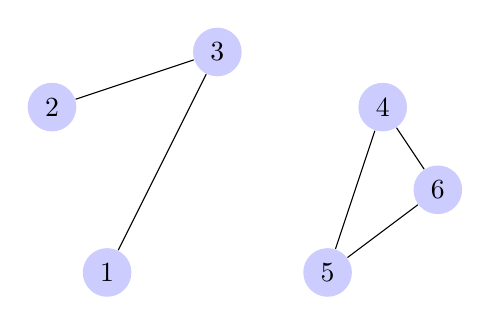
\begin{tikzpicture}
			[scale=.35,auto=left,every node/.style={circle,fill=blue!20}]
			\node (n1) at (0,0) {1};
			\node (n2) at (-2,6)  {2};
			\node (n3)  at (4,8) {3};
			\node (n4) at (10,6)  {4};
			\node (n5) at (8,0)  {5};
			\node (n6) at (12,3)  {6};
			
			\foreach \from/\to in 
			{n5/n4, n2/n3,  n3/n1, n6/n4, n6/n5}
			\draw (\from) -- (\to);
			\end{tikzpicture}
			\caption{A graph $G$ with two disconnected components $G_1$ and $G_2$}
			\label{fig:Disconnected}
		\end{figure}
\end{example}


\begin{example}
	In figure \ref{fig:Forest}, we have a graph $F$. where we have:\\ \\$V=\{v_1,v_2,v_3,v_4,v_5, v_6\}$
	\\
	\\$E=\{ (v_1, v_3) , (v_2, v_3), (v_3,v_4), (v_4,v_6),(v_4,v_5)\}$\\
	\\
	This example is a forest as it contains no cycles.
	\begin{figure}[h!]
		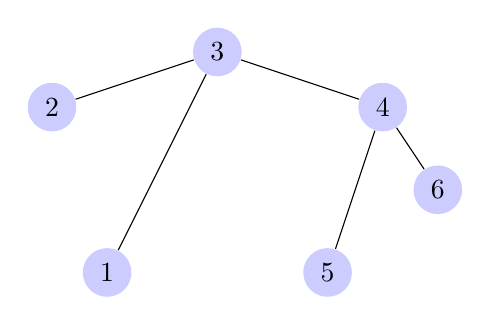
\begin{tikzpicture}
		[scale=.35,auto=left,every node/.style={circle,fill=blue!20}]
		\node (n1) at (0,0) {1};
		\node (n2) at (-2,6)  {2};
		\node (n3)  at (4,8) {3};
		\node (n4) at (10,6)  {4};
		\node (n5) at (8,0)  {5};
		\node (n6) at (12,3)  {6};
		
		\foreach \from/\to in 
		{n5/n4, n2/n3,  n3/n1, n3/n4, n6/n4}
		\draw (\from) -- (\to);
		\end{tikzpicture}
		\caption{A graph $F$ which is a forest (note that this is also a tree)}
		\label{fig:Forest}
	\end{figure}
\end{example}

\begin{example}
	In figure \ref{fig:ForestTwo}, we have a graph $F$. where we have:\\ \\$V=\{v_1,v_2,v_3,v_4,v_5, v_6\}$
	\\
	\\$E=\{ (v_1, v_3) , (v_2, v_3), (v_4,v_6),(v_4,v_5)\}$\\
	\\
	This example is a forest as it contains no cycles.\\
	\\
	 Unlike our previous example, it is not a tree as it contains two disconnected components.
	\begin{figure}[h!]
		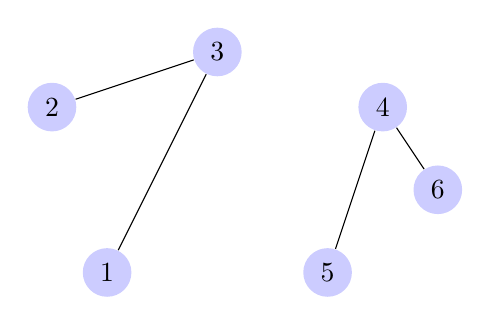
\begin{tikzpicture}
		[scale=.35,auto=left,every node/.style={circle,fill=blue!20}]
		\node (n1) at (0,0) {1};
		\node (n2) at (-2,6)  {2};
		\node (n3)  at (4,8) {3};
		\node (n4) at (10,6)  {4};
		\node (n5) at (8,0)  {5};
		\node (n6) at (12,3)  {6};
		
		\foreach \from/\to in 
		{n5/n4, n2/n3,  n3/n1, n6/n4}
		\draw (\from) -- (\to);
		\end{tikzpicture}
		\caption{A graph $F$ which is a forest but not a tree}
		\label{fig:ForestTwo}
	\end{figure}
\end{example}

\begin{example}
	In figure \ref{fig:Digraph}, we see our first example of a digraph. In this example, there are two edges which can only be traversed from $v_1$ to $v_2$, one edge which can be traversed in from $v_1$ to $v_2$ and $v_2$ to $v_1$. \\
	\\
	We also see there is an edge from $v_2$ to itself.\\
	\\
	\begin{figure}[h!]
		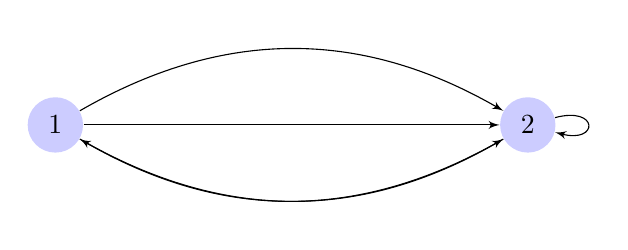
\begin{tikzpicture}
		[scale=1,auto=left, edge/.style = {->,> = latex'}, every vertex/.style={circle,fill=blue!20}]
		\node[vertex][style={circle,fill=blue!20}] (a1) at (0,0) {1};
		\node[vertex][style={circle,fill=blue!20}] (a2) at (6,0) {2};
		
		\draw[edge] (a1) to[bend left] (a2);
		\draw[edge] (a1) to (a2);
		\draw[edge] (a2) to[bend left] (a1);
		\draw[edge] (a1) to[bend right] (a2);
		\draw[edge] (a2) to[loop right,thick] (a2);
		
		\end{tikzpicture}
		\caption{A digraph with a self-connected vertex}
		\label{fig:Digraph}
	\end{figure}
\end{example}

\pagebreak
\section{The Konigsberg Bridges}
\noindent We've seen a few examples of graphs, and different definitions concerning graphs; in this section, we motivate their study by examining the origin of Graph Theory touched upon in Lecture 16. \\
\\
In 1736, a contemporary open problem was to determine if it was possible to visit each of the four landmasses in the city of Konigsberg, which were connected as shown in figure \ref{fig:Konigsberg} by seven bridges, crossing each bridge only once (in modern terms, as introduced in the definitions above, the question was if a Eulerian path exists on Konigsberg's graph topology).
\begin{figure}[h!]
	\centering
	\includegraphics[width=0.4\linewidth]{KonigsbergGraph}
	\caption{The Bridges of Konigsberg	\href{https://www.maa.org/press/periodicals/convergence/leonard-eulers-solution-to-the-konigsberg-bridge-problem}{Source: The MAA}}
	\label{fig:Konigsberg}
\end{figure}

\noindent One of the key challenge in this problem for contemporary mathematicians was that they lacked suitable tools for analysing this type of problem, and converting it into one which could be tackled using numerical techniques and algorithms.\\
\\
Euler's key insight to solve this problem was in recognising that the problem could be abstracted from the physical characteristics of the problem, and observing that the key of the problem was in how each landmass was connected, and recognising that landmasses could be represented by nodes with edges (i.e. the bridges) connecting those points. By abstracting the problem, it can be represented using the terminology and notation above with the graph in figure \ref{fig:KonigGraph} (although it is worth noting that this representation followed much later).
\begin{figure}[h!]
	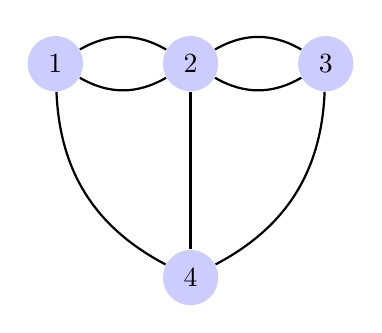
\begin{tikzpicture}
				
			 \tikzset{VertexStyle/.style = {shape          = circle,
					fill     = blue!20,
					minimum size   = 20 pt}}
				
			\tikzset{EdgeStyle/.style   = {thick}}
				
			\node[VertexStyle](1){1};
			\node[VertexStyle,right=of 1](2){2};
			\node[VertexStyle,right=of 2](3){3};
			\node[VertexStyle,below= 2 cm of 2](4){4};  
			   
			\draw[EdgeStyle](2) to node {}(4);
			\tikzset{EdgeStyle/.append style = {bend right}}
			\draw[EdgeStyle](1) to node {}(2);
			\draw[EdgeStyle](2) to node {}(1);
			\draw[EdgeStyle](2) to node {}(3);
			\draw[EdgeStyle](3) to node {}(2);
			\draw[EdgeStyle](1) to node {}(4);
			\draw[EdgeStyle](4) to node {}(3);
			\end{tikzpicture}
		\caption{The Bridges of Konigsberg in a Graph}
		\label{fig:KonigGraph}
\end{figure}
\noindent The core of Euler's solution was in recognising that we had an even number of vertices, an odd number of edges, and a degree sequence incompatabile with an Eulerian cycle. The 'algorithm' which Euler described in demonstrating that there was no solution was that if we enter a vertex on an edge, we can 'burn' that edge from the graph as that edge cannot be traversed again. Therefore, we must exit the vertex on a different edge. Hence that vertex must have an even number of edges to facilitate 'entering' and 'exiting' the vertex on unique edges. Therefore in a Eulerian Path there can be at most two vertices with odd degree, and furthermore we therefore have that in a connected graph with an Eulerian cycle all vertices must have an even degree, yet in the Konigsberg Graph above neither of these conditions are met as $d(v_1)=d(v_3)=d(v_4)=3$, $d(v_2)=5$ and hence there is no Eulerian path or Eulerian cycle within this graph.

\pagebreak
\section{Modern Applications of Graphs}
\noindent Since Euler's 1736 paper establishing the field, Graph Theory has grown immeasurably from that original paper. In a modern context, the graph data structure which serves as a representation of how two items connect/relate in an abstract manner has had a fundamental impact in how key aspects of modern society function. In this section, we will examine three key examples before fundamentally looking at the Graph ADT and converting the mathematical definitions of a graph into a data structure. In particular, we will examine:
\begin{itemize}
	\item The usage of graphs in PageRank.
	\item The usage of graphs in Social Network Analysis.
	\item The usage of graphs in City Modelling.
\end{itemize}

\begin{example}
	One of the most prominent examples of Graphs in a modern context is in its widespread usage in search engine optimisation, most notably in Google's PageRank algorithm (detailed on \href{https://neo4j.com/docs/graph-data-science/current/algorithms/page-rank}{Neo4J's Overview of PageRank}). A key aspect in this algorithm, which is used for determining the 'importance' of web pages and where they should be ranked in relation to search engine queries, is that the world wide web is viewed as a graph wherein each node is a webpage (or website) and edges between notes are formed from webpages linking to other webpages. A sample of this is provided in \ref{fig:SiteGraph}. At a high level, in this algorithm, pages are weighted based on the relative importance of other pages which are linking to them, the quantity of pages linking to them, and a damping factor. 
	\begin{figure}[h!]
		\centering
		\includegraphics[width=0.8\linewidth]{page-rank}
		\caption{A Site Graph \href{https://neo4j.com/docs/graph-data-science/current/algorithms/page-rank}{Source: Neo4J}}
		\label{fig:SiteGraph}
	\end{figure}
	\noindent This algorithm has played an incredibly important role not only in the establishment of Google as one of the largest companies worldwide, but has played a critical role in how we browse the world wide web today, and the Graph Data Structure plays a fundamental role in how this algorithm works.
\end{example}

\begin{example}
	A prominent usage of graph data types is in Social Network Analysis, such as that featured in \href{http://social-dynamics.org/twitter-network-data/}{Analysing Twitter Network Data}. The relation of accounts of follow or follower or friends which is commonly featured on social media websites can be represented as a digraph (in the case of a follow and follower dynamic) or simply connected graph (in the case of a mutual dynamic). An example of this concerning Twitter data can be visualised in the below graph:
	
	\begin{figure}[h!]
		\centering
		\includegraphics[width=0.5\linewidth]{pjlambersonTwitter10_16_12}
		\caption{Twitter Relation Graph \href{http://social-dynamics.org/twitter-network-data/}{Source: Social Dynamics}}
		\label{fig:TwitterGraph}
	\end{figure}
\noindent This view of follower/friend dynamic is often used by social media sites in order to develop recommender systems which highlight specific individuals to follow. Twitter for example utilises a modified PageRank algorithm looking at their own follower graph to recommend particular users to follow to other users on the site. Similarly, within eCommerce websites, page-relation graphs combined with clickstream data can be used to weigh personalised product recommendations to users without known preference behaviour in a similar manner to how people are 'recommended' connections on social media sites.
\end{example}

\begin{example}
	The final example which will be touched upon is how graphs have a significant role in the area of urban planning/ Graphs can be used to model the topology of a city, such as \href{https://core.ac.uk/download/pdf/132348208.pdf}{Agryzkov, Oliver, et al's paper on modelling Alicante}, or by Google Maps in modelling the shortest paths between various points on maps within or between cities/countries. By modelling roads as edges and intersections as vertices (or alternative representations depending on the goal) and weighing these roads based on certain conditions (such as distance, time to travel at the speed limit, traffic, etc.) key insight can be gain into how traffic flows between cities and in what routes are considered optimal between two points within the city. This can play an important role both in how cities are designed, and also in how we navigate through cities while assisted by technology.
\end{example}

\pagebreak
\section{The Graph ADT and its Operations}
\noindent Now that we have seen graphs in a more mathematical concept, examined the historic usage, and looked at modern examples of graphs as touched upon the Lecture 16, for the remainer of this paper we will direct our attention towards the Graph ADT.\\
\\
As mentioned in definition \ref{GADT}, in the Graph ADT we consider both directed graphs and undirected graphs. In lecture 16, the key focus was on simple undirected graphs and therefore this will form the basis of the remainder. A graph has a few key operations which we will examine from an adjacency matrix perspective (assuming valid entries) perspective, and to examine them we will consider once again the following graph on which we will perform the key operation:
	\begin{figure}[h!]
	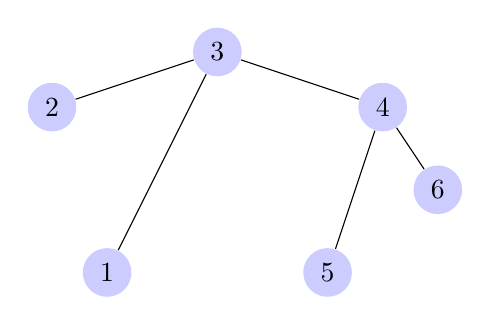
\begin{tikzpicture}
	[scale=.35,auto=left,every node/.style={circle,fill=blue!20}]
	\node (n1) at (0,0) {1};
	\node (n2) at (-2,6)  {2};
	\node (n3)  at (4,8) {3};
	\node (n4) at (10,6)  {4};
	\node (n5) at (8,0)  {5};
	\node (n6) at (12,3)  {6};
	
	\foreach \from/\to in 
	{n5/n4, n2/n3,  n3/n1, n3/n4, n6/n4}
	\draw (\from) -- (\to);
	\end{tikzpicture}
	\caption{A graph $F$}
	\label{fig:ForestV2}
\end{figure}

\newpage
\begin{oper}
	\textbf{adjacent(G,x,y)}
	This tests whether x and y are adjacent (i.e. there exists an edge between x and y). \\
	\\
	The time complexity of the algorithm below is $\mathrm{O}(1)$.\\
	\\
	On our example:
	\begin{itemize}
		\item adjacent$(F,v_1,v_2) = $ False.
		\item adjacent$(F,v_1,v_3) = $ True.
		\item adjacent$(F,v_2,v_3) = $ True.
		\item adjacent$(F,v_4,v_1) = $ False.
	\end{itemize}

	\begin{figure}[h!]
	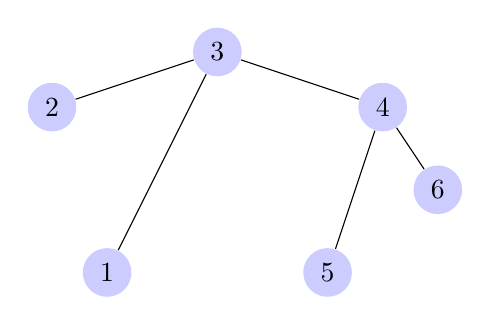
\begin{tikzpicture}
	[scale=.35,auto=left,every node/.style={circle,fill=blue!20}]
	\node (n1) at (0,0) {1};
	\node (n2) at (-2,6)  {2};
	\node (n3)  at (4,8) {3};
	\node (n4) at (10,6)  {4};
	\node (n5) at (8,0)  {5};
	\node (n6) at (12,3)  {6};
	
	\foreach \from/\to in 
	{n5/n4, n2/n3,  n3/n1, n3/n4, n6/n4}
	\draw (\from) -- (\to);
	\end{tikzpicture}
	\caption{$F$}
	\label{fig:ForestDupe1}
\end{figure}

\pagebreak
\begin{algorithm}[H]
	\SetAlgoLined
	\KwIn{G,a,b}
	\KwResult{If $ab \in E$ then True Else False}
	\KwOut{True/False}
	\If{$G[a][b]=1$}{
		Return True
	}
	Return False
	\caption{adjacent}
\end{algorithm}
\end{oper}

\newpage
\begin{oper}
	\textbf{neighbours(G,x)}\\
	This lists all vertices $y$, where $x \neq y$ such that there exists an edge $xy$ (please refer to \href{https://mathworld.wolfram.com/GraphNeighborhood.html}{Wolfram where Brower et al.'s non-equal requirement is specified}; the \textbf{neighbourhood} of a vertex includes itself, however the \textbf{neighbours} of a vertex does not - although this can depend on the implementation).\\
	\\
	The time complexity of the algorithm below is $\mathrm{O}(n)$.\\
	\\
	
	\begin{itemize}
	\item neighbours$(F,v_1) =\{v_3\}$.
	\item neighbours$(F,v_2) = \{v_3\}$.
	\item neighbours$(F,v_3) = \{v_1,v_2,v_4\}$.
	\item neighbours$(F,v_4) = \{v_5,v_6,v_3\}$.
\end{itemize}

	\begin{figure}[h!]
	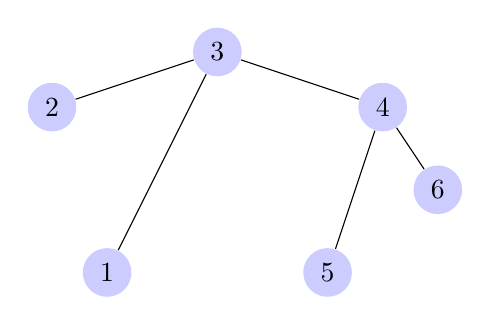
\begin{tikzpicture}
	[scale=.35,auto=left,every node/.style={circle,fill=blue!20}]
	\node (n1) at (0,0) {1};
	\node (n2) at (-2,6)  {2};
	\node (n3)  at (4,8) {3};
	\node (n4) at (10,6)  {4};
	\node (n5) at (8,0)  {5};
	\node (n6) at (12,3)  {6};
	
	\foreach \from/\to in 
	{n5/n4, n2/n3,  n3/n1, n3/n4, n6/n4}
	\draw (\from) -- (\to);
	\end{tikzpicture}
	\caption{$F$}
	\label{fig:Dupe2}
\end{figure}
\pagebreak
\begin{algorithm}[H]
	\SetAlgoLined
	\KwIn{G,a}
	\KwResult{A vertex $a$ is added if it is not already present}
	\KwOut{$N:=\{v \in V : uv \in E\}$}
	$N=\{\}$\\
	\For{$v$ in $G$}
	{
		\If{$G[v][a]=1, a\neq v$}
		{
				$N.add(v)$\\
			}
	}
	Return $N$
	\caption{neighbours}
\end{algorithm}


\end{oper}

\newpage
\begin{oper}
	\textbf{add\_vertex(G,x)}\\
	This adds the vertex G to the Graph ADT.\\
	\\
		The time complexity of the algorithm below is $\mathrm{O}(1)$ (note: this is assuming the vertex is not present already).\\
	\\
	\begin{itemize}
	\item add\_vertex$(F,v_1)$\\
		\begin{figure}[h!]
			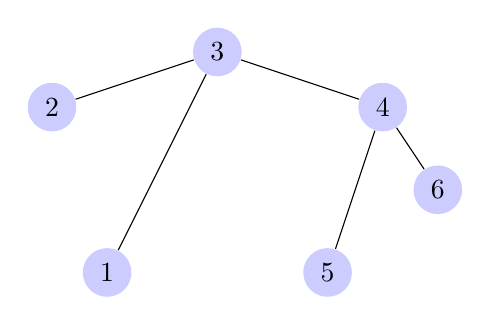
\begin{tikzpicture}
			[scale=.35,auto=left,every node/.style={circle,fill=blue!20}]
			\node (n1) at (0,0) {1};
			\node (n2) at (-2,6)  {2};
			\node (n3)  at (4,8) {3};
			\node (n4) at (10,6)  {4};
			\node (n5) at (8,0)  {5};
			\node (n6) at (12,3)  {6};
			
			\foreach \from/\to in 
			{n5/n4, n2/n3,  n3/n1, n3/n4, n6/n4}
			\draw (\from) -- (\to);
			\end{tikzpicture}
		\caption{$F$ after adding v\_1 - No change as $v_1$ exists}
		\label{fig:AddV}
	\end{figure}

	\item add\_vertex$(F,v_7)$.\\
		\begin{figure}[h!]
	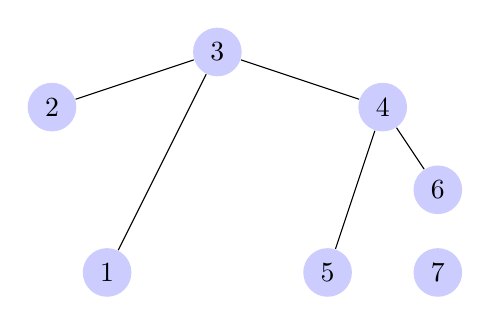
\begin{tikzpicture}
	[scale=.35,auto=left,every node/.style={circle,fill=blue!20}]
	\node (n1) at (0,0) {1};
	\node (n2) at (-2,6)  {2};
	\node (n3)  at (4,8) {3};
	\node (n4) at (10,6)  {4};
	\node (n5) at (8,0)  {5};
	\node (n6) at (12,3)  {6};
	\node (n7) at (12,0)  {7};
	
	\foreach \from/\to in 
	{n5/n4, n2/n3,  n3/n1, n3/n4, n6/n4}
	\draw (\from) -- (\to);
	\end{tikzpicture}
	\caption{$F$ after adding v\_7}
	\label{fig:ForestV3}
\end{figure}


	\item add\_vertex$(F,v_8)$.\\
			\begin{figure}[h!]
		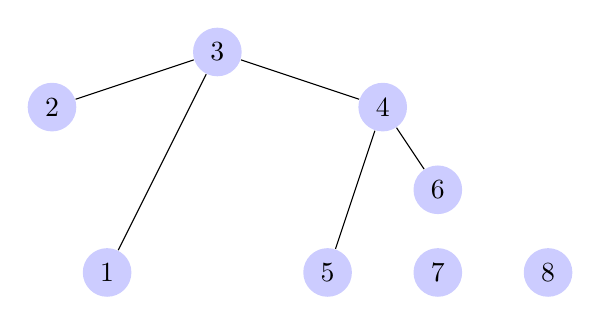
\begin{tikzpicture}
		[scale=.35,auto=left,every node/.style={circle,fill=blue!20}]
		\node (n1) at (0,0) {1};
		\node (n2) at (-2,6)  {2};
		\node (n3)  at (4,8) {3};
		\node (n4) at (10,6)  {4};
		\node (n5) at (8,0)  {5};
		\node (n6) at (12,3)  {6};
		\node (n7) at (12,0)  {7};
		\node (n8) at (16,0)  {8};
		
		\foreach \from/\to in 
		{n5/n4, n2/n3,  n3/n1, n3/n4, n6/n4}
		\draw (\from) -- (\to);
		\end{tikzpicture}
		\caption{$F$ after adding v\_7 and v\_8}
		\label{fig:ForestElse}
	\end{figure}
\end{itemize}
\pagebreak
\begin{algorithm}[H]
	\SetAlgoLined
	\KwIn{G,a}
	\KwResult{A vertex $a$ is added}
	\KwOut{None}
	\For{$v$ in $G$}
		{$G[v][a]=0$\\
		$G[a][v]=0$\\
		}
	\caption{add\_vertex}
\end{algorithm}

\end{oper}

\newpage
\begin{oper}
	\textbf{add\_edge(G,x,y)}\\
	Adds an edge between x and y if there is not already one present.\\	
	\\
	The time complexity of the algorithm below is $\mathrm{O}(1)$.\\
	\\
	
	\begin{itemize}
	\item add\_edge$(F,v_6,v_7)$.\\
				\begin{figure}[h!]
		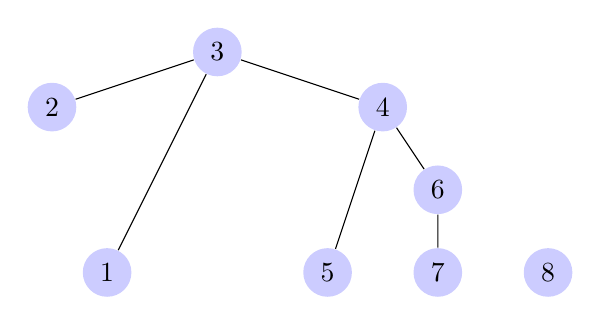
\begin{tikzpicture}
		[scale=.35,auto=left,every node/.style={circle,fill=blue!20}]
		\node (n1) at (0,0) {1};
		\node (n2) at (-2,6)  {2};
		\node (n3)  at (4,8) {3};
		\node (n4) at (10,6)  {4};
		\node (n5) at (8,0)  {5};
		\node (n6) at (12,3)  {6};
		\node (n7) at (12,0)  {7};
		\node (n8) at (16,0)  {8};
		
		\foreach \from/\to in 
		{n5/n4, n2/n3,  n3/n1, n3/n4, n6/n4, n6/n7}
		\draw (\from) -- (\to);
		\end{tikzpicture}
		\caption{$F$ after adding v\_7 and v\_8 and edge}
		\label{fig:ForestV4}
	\end{figure}
	\item add\_edge$(F,v_6,v_7)$.
		\begin{figure}[h!]
			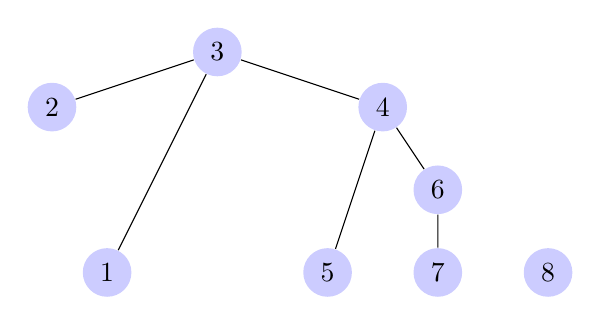
\begin{tikzpicture}
			[scale=.35,auto=left,every node/.style={circle,fill=blue!20}]
			\node (n1) at (0,0) {1};
			\node (n2) at (-2,6)  {2};
			\node (n3)  at (4,8) {3};
			\node (n4) at (10,6)  {4};
			\node (n5) at (8,0)  {5};
			\node (n6) at (12,3)  {6};
			\node (n7) at (12,0)  {7};
			\node (n8) at (16,0)  {8};
			
			\foreach \from/\to in 
			{n5/n4, n2/n3,  n3/n1, n3/n4, n6/n4, n6/n7}
			\draw (\from) -- (\to);
			\end{tikzpicture}
			\caption{$F$ No change as it exists}
			\label{fig:ForestV5}
		\end{figure}
	\item add\_edge$(F,v_7,v_8)$.
			\begin{figure}[h!]
		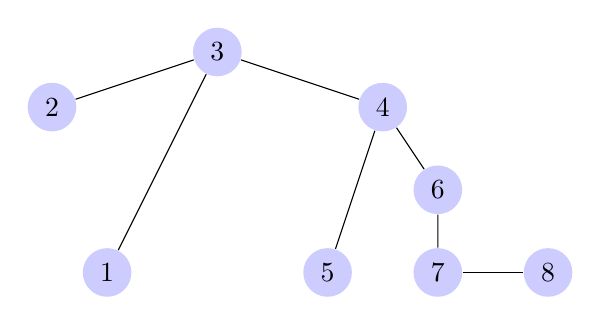
\begin{tikzpicture}
		[scale=.35,auto=left,every node/.style={circle,fill=blue!20}]
		\node (n1) at (0,0) {1};
		\node (n2) at (-2,6)  {2};
		\node (n3)  at (4,8) {3};
		\node (n4) at (10,6)  {4};
		\node (n5) at (8,0)  {5};
		\node (n6) at (12,3)  {6};
		\node (n7) at (12,0)  {7};
		\node (n8) at (16,0)  {8};
		
		\foreach \from/\to in 
		{n5/n4, n2/n3,  n3/n1, n3/n4, n6/n4, n6/n7,n7/n8}
		\draw (\from) -- (\to);
		\end{tikzpicture}
		\caption{$F$ Edge added}
		\label{fig:ForestV6}
	\end{figure}
\end{itemize}
\pagebreak
\begin{algorithm}[H]
	\SetAlgoLined
	\KwIn{G,a,b}
	\KwResult{An edge $ab$ is added if it does not already exist}
	\KwOut{None}
	 G[a][b]=1\\
	 G[b][a]=1
	Return
		\caption{add\_edge}
\end{algorithm}

\end{oper}

\pagebreak
\begin{oper}
	\textbf{remove\_edge(G,x,y)}\\
	Removes the edge between x and y if present	\\
	\\
	The time complexity of the algorithm below is $\mathrm{O}(1)$ assuming x and y are not in G.\\
	\\
	
	\begin{itemize}
	\item remove\_edge$(F,v_8,v_6)$.\\
				\begin{figure}[h!]
		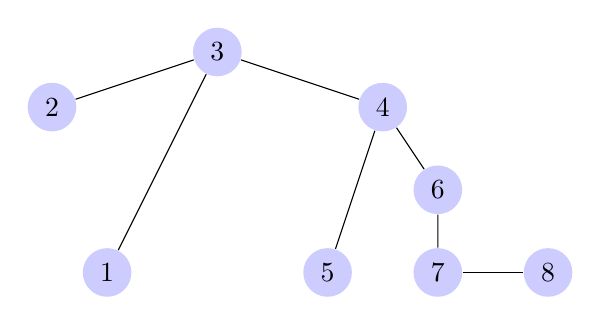
\begin{tikzpicture}
		[scale=.35,auto=left,every node/.style={circle,fill=blue!20}]
		\node (n1) at (0,0) {1};
		\node (n2) at (-2,6)  {2};
		\node (n3)  at (4,8) {3};
		\node (n4) at (10,6)  {4};
		\node (n5) at (8,0)  {5};
		\node (n6) at (12,3)  {6};
		\node (n7) at (12,0)  {7};
		\node (n8) at (16,0)  {8};
		
		\foreach \from/\to in 
		{n5/n4, n2/n3,  n3/n1, n3/n4, n6/n4, n6/n7,n7/n8}
		\draw (\from) -- (\to);
		\end{tikzpicture}
		\caption{$F$ Edge doesnt exist so no change}
		\label{fig:ForestV8}
	\end{figure}
	\item remove\_edge$(F,v_8,v_7)$.\\
				\begin{figure}[h!]
		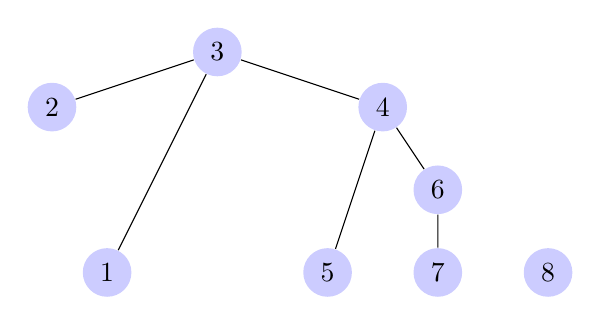
\begin{tikzpicture}
		[scale=.35,auto=left,every node/.style={circle,fill=blue!20}]
		\node (n1) at (0,0) {1};
		\node (n2) at (-2,6)  {2};
		\node (n3)  at (4,8) {3};
		\node (n4) at (10,6)  {4};
		\node (n5) at (8,0)  {5};
		\node (n6) at (12,3)  {6};
		\node (n7) at (12,0)  {7};
		\node (n8) at (16,0)  {8};
		
		\foreach \from/\to in 
		{n5/n4, n2/n3,  n3/n1, n3/n4, n6/n4, n6/n7}
		\draw (\from) -- (\to);
		\end{tikzpicture}
		\caption{$F$ Edge removed}
		\label{fig:ForestV7}
	\end{figure}
	
	\item remove\_edge$(F,v_6,v_7)$.\\
					\begin{figure}[h!]
		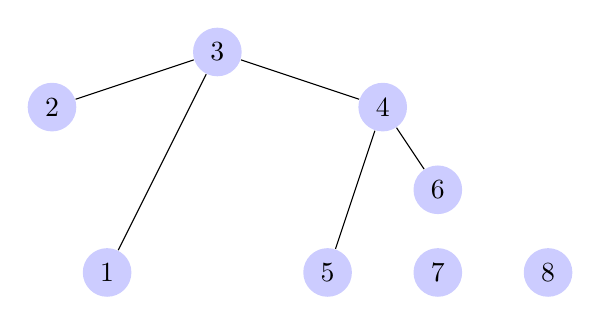
\begin{tikzpicture}
		[scale=.35,auto=left,every node/.style={circle,fill=blue!20}]
		\node (n1) at (0,0) {1};
		\node (n2) at (-2,6)  {2};
		\node (n3)  at (4,8) {3};
		\node (n4) at (10,6)  {4};
		\node (n5) at (8,0)  {5};
		\node (n6) at (12,3)  {6};
		\node (n7) at (12,0)  {7};
		\node (n8) at (16,0)  {8};
		
		\foreach \from/\to in 
		{n5/n4, n2/n3,  n3/n1, n3/n4, n6/n4}
		\draw (\from) -- (\to);
		\end{tikzpicture}
		\caption{$F$ Edge removed}
		\label{fig:ForestV7}
	\end{figure}
\end{itemize}
\pagebreak
\begin{algorithm}[H]
	\SetAlgoLined
	\KwIn{G,a,b}
	\KwResult{An edge $ab$ is removed.}
	\KwOut{None}
		$G[a][b]=0$\\
		$G[b][a]=0$\\
		Return
	\caption{remove\_edge}
\end{algorithm}
\end{oper}

\pagebreak
\begin{oper}
	\textbf{remove\_vertex(G,x)}\\
	Removes x from the vertex set if present.\\
	\\
	The time complexity of the algorithm below is $\mathrm{O}(n)$ assuming x is in G.\\
	\\
	
	\begin{itemize}
		\item remove\_vertex$(F,v_8)$.\\
							\begin{figure}[h!]
			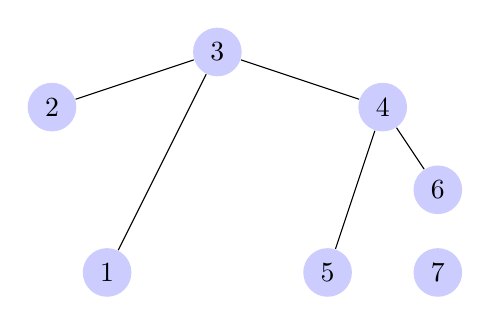
\begin{tikzpicture}
			[scale=.35,auto=left,every node/.style={circle,fill=blue!20}]
			\node (n1) at (0,0) {1};
			\node (n2) at (-2,6)  {2};
			\node (n3)  at (4,8) {3};
			\node (n4) at (10,6)  {4};
			\node (n5) at (8,0)  {5};
			\node (n6) at (12,3)  {6};
			\node (n7) at (12,0)  {7};
			
			\foreach \from/\to in 
			{n5/n4, n2/n3,  n3/n1, n3/n4, n6/n4}
			\draw (\from) -- (\to);
			\end{tikzpicture}
			\caption{$F$ Vertex removed}
			\label{fig:ForestV9}
		\end{figure}
		\item remove\_vertex$(F,v_8) $.\\
									\begin{figure}[h!]
			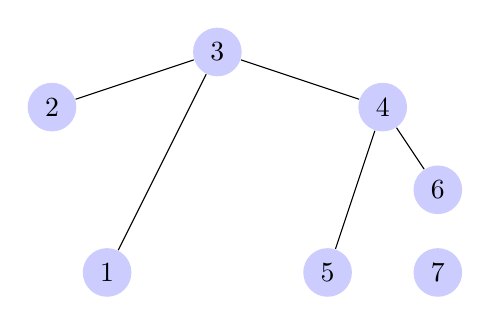
\begin{tikzpicture}
			[scale=.35,auto=left,every node/.style={circle,fill=blue!20}]
			\node (n1) at (0,0) {1};
			\node (n2) at (-2,6)  {2};
			\node (n3)  at (4,8) {3};
			\node (n4) at (10,6)  {4};
			\node (n5) at (8,0)  {5};
			\node (n6) at (12,3)  {6};
			\node (n7) at (12,0)  {7};
			
			\foreach \from/\to in 
			{n5/n4, n2/n3,  n3/n1, n3/n4, n6/n4}
			\draw (\from) -- (\to);
			\end{tikzpicture}
			\caption{$F$ No change}
			\label{fig:ForestV9}
			\end{figure}
		
		\item remove\_vertex$(F,v_7)$.\\
			\begin{figure}[h!]
			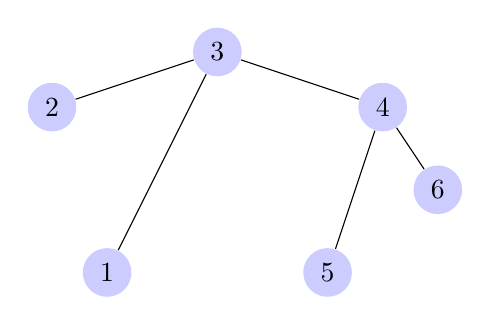
\begin{tikzpicture}
			[scale=.35,auto=left,every node/.style={circle,fill=blue!20}]
			\node (n1) at (0,0) {1};
			\node (n2) at (-2,6)  {2};
			\node (n3)  at (4,8) {3};
			\node (n4) at (10,6)  {4};
			\node (n5) at (8,0)  {5};
			\node (n6) at (12,3)  {6};
			
			\foreach \from/\to in 
			{n5/n4, n2/n3,  n3/n1, n3/n4, n6/n4}
			\draw (\from) -- (\to);
			\end{tikzpicture}
			\caption{$F$ Vertex removed}
			\label{fig:ForestV9}
			\end{figure}
	\end{itemize}
\pagebreak
\begin{algorithm}[H]
\SetAlgoLined
\KwIn{G,a}
\KwResult{A vertex $a$ is removed.}
\KwOut{None}
		\For{v in G}
			{$G[v][a]=0$
			\\$G[a][v]=0$}
\caption{remove\_vertex}
\end{algorithm}
\end{oper}

\pagebreak
\section{Graph Representation}\label{repr}
\noindent Having seen the Graph ADT and examples of operations on the Graph ADT, we turn our attention to how graphs may be represented.\\
\\
There are two key methods which are used to represent graphs in a computer data structure.
\begin{itemize}
	\item Adjacency Lists
	\item Adjacency Matrices
\end{itemize}

\noindent While we will examine both formats, in choosing which format to use to represent the graph the key the key element is in the ratio between the size and order of the graph.\\
\\
When  $|E| < < |V|^2$, i.e. the graph is sparse, then adjacency lists provide a more compact representation. \\
\\
When  $|E| \approxeq |V|^2$ (note that in an undirected simple graph which is not a multigraph we trivially have $|E|<=(|V|)(|V|-1)$), i.e. the graph is dense, then adjacency matrices provide a better representation method.

\begin{definition}
	Let $G=(V,E)$ be a graph where $V=\{v_1,\dots,v_n\}$.\\
	\\
	Then the Adjacency Matrix, with respect to the labelling, denoted $A(G)$ with $ A(G) \in M_n(\mathbb{Z})$ is defined by:\\
	\\
	$A(G)=(a_{i,j})_{i,j = 1}^{n}$\\
	\\
	where\\
	\\
	$a_{i,j} := | \{v_{i}v_{j} \in E\}| =$ Number of edges connecting $v_{i}$ and $v_{j}$\\
	\\
	\noindent This is stored using a $|V||V|$ array.
\end{definition}

\begin{remark}
	This definition can be adapted to the case of weighted graphs where\\ $(a_{i,j}):= \sum\limits_{v_iv_j \in E} w(v_i,v_j)$ i.e. the sum of weights of edges connecting $v_i$ and $v_j$.
\end{remark}

\begin{example}
	Consider the graph:
		\begin{figure}[h!]
		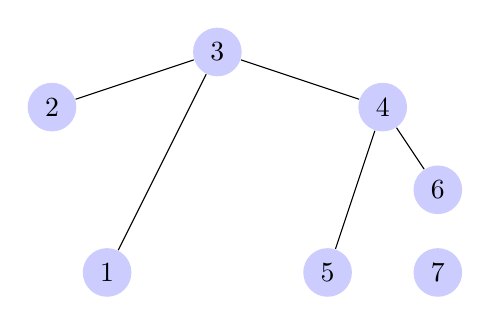
\begin{tikzpicture}
		[scale=.35,auto=left,every node/.style={circle,fill=blue!20}]
		\node (n1) at (0,0) {1};
		\node (n2) at (-2,6)  {2};
		\node (n3)  at (4,8) {3};
		\node (n4) at (10,6)  {4};
		\node (n5) at (8,0)  {5};
		\node (n6) at (12,3)  {6};
		\node (n7) at (12,0)  {7};
		
		\foreach \from/\to in 
		{n5/n4, n2/n3,  n3/n1, n3/n4, n6/n4}
		\draw (\from) -- (\to);
		\end{tikzpicture}
		\caption{$G$ Example graph}
		\label{fig:ForestV9}
	\end{figure}
	
The adjacency matrix of this graph is:
\begin{math}
A(G) = 
\begin{pmatrix}
		0 & 
		0 & 
		1 & 
		0 & 
		0 & 
		0 & 
		0
		\\ 
		0& 
		 0&  
		 1& 
		 0& 
		 0& 
		 0& 
		 0 
		 \\
		 1 & 
		 1  &  
		 0 & 
		 1 & 
		 0 & 
		 0& 
		 0 
		 \\
		 0& 
		 0 &  
		 1& 
		 0& 
		 1& 
		 1& 
		 0 
		 \\
		 0& 
		 0&  
		 0& 
		 1& 
		 0& 
		 0& 
		 0 
		 \\
		 0& 
		 0&  
		 0& 
		 1& 
		 0& 
		 0& 
		 0 
		 \\
		 0& 
		 0 &  
		 0& 
		 0& 
		 0& 
		 0& 
		 0 
	\end{pmatrix} 
\end{math}
\end{example}


\begin{definition}
	Let $G=(V,E)$ be a graph. \\
	\\
	The adjacency list of a vertex $v_l$ is an array with:
	
	$(a_{l,j})_{j \in \{u \in V : v_lu \in E\}}$\\
	\\
	G is then the union of each vertices' adjacency list.
\end{definition}

\begin{example}
	Consider the graph:
	\begin{figure}[h!]
		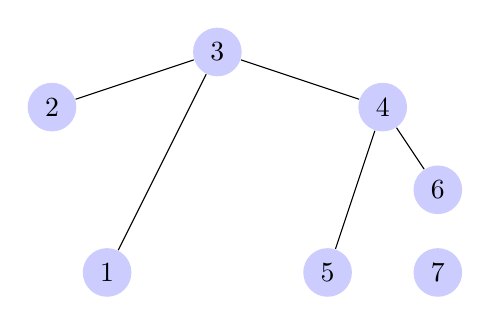
\begin{tikzpicture}
		[scale=.35,auto=left,every node/.style={circle,fill=blue!20}]
		\node (n1) at (0,0) {1};
		\node (n2) at (-2,6)  {2};
		\node (n3)  at (4,8) {3};
		\node (n4) at (10,6)  {4};
		\node (n5) at (8,0)  {5};
		\node (n6) at (12,3)  {6};
		\node (n7) at (12,0)  {7};
		
		\foreach \from/\to in 
		{n5/n4, n2/n3,  n3/n1, n3/n4, n6/n4}
		\draw (\from) -- (\to);
		\end{tikzpicture}
		\caption{$G$ Example graph}
		\label{fig:Forest9}
	\end{figure}
	
	The adjacency list representation of this graph is:

	\begin{table}[h]
		\begin{tabular}{|c|c|}
			\hline
		\textbf{Vertex}&\textbf{List}\\
		\hline
		$v_1$&$v_3$\\
		\hline
		$v_2$&$v_3$\\
		\hline
		$v_3$&$v_1,v_2,v_4$\\
		\hline
		$v_4$&$v_5,v_6,v_3$\\
		\hline
		$v_5$&$v_4$\\
		\hline
		$v_6$&$v_4$\\
		\hline
		$v_7$&\\
		\hline
		\end{tabular}
	\end{table} 
\end{example}

\begin{remark}
	Both of these have different positives and benefits. The matrix representation is arguably intuitively easier to understand, however the space complexity remains constant at $|V|^2$ as it must store an entry for each node. In a sparse matrix, this means a lot of information is 'needlessly' stored. In the case of the adjacency list, while it may not be as inuitively easy to understand, it does have the benefit of requiring much less storage if the graph is particularly sparse. The operation performance also has an impact; in an adjacency list, returning the neighbours of a node is as simple as returning the list for a given node while in an adjacency matrix structure the entire row or column must be scanned to determine the adjacent vertices. Similarly, a matrix form may allow for a greater degree of algebraic techniques to be more easily applied to the graph (e.g. spectral analysis).
\end{remark}

\pagebreak
\section{DFS and BFS}
\noindent The final component of Lecture 16 was examining the depth-first search (DFS) and breadth-first search (BFS) algorithm associated with graphs. Both methods are algorithms for exploring a graph in order to identify if a path between two nodes exist in a graph.\\
\\
We will examine both of these algorithms through examples, but first we recall these algorithms from lecture 16:\\
\\

\begin{figure}[h!]
	\centering
	\includegraphics[width=0.5\linewidth]{dfs}
	\caption{DFS Algorithm from Lecture 16}
	\label{fig:Konigsberg}
\end{figure}
\noindent In the DFS algorithm, we start at a given vertex and explore all paths from that vertex, following paths based on lexicographical ordering in the instance that a vertex has multiple neighbours.\\
\\
One important component missing in the DFS algorithm highlighted in lecture 16 is that this particular version of an algorithm will only search from a given starting node. For a complete traversal, to account for the instance where we have $K(G)>1$, we need to run this algorithm on starting with one node in all components of $G$.
\\
\pagebreak
\begin{example}
	Consider the graph:\\
	\begin{figure}[h!]
		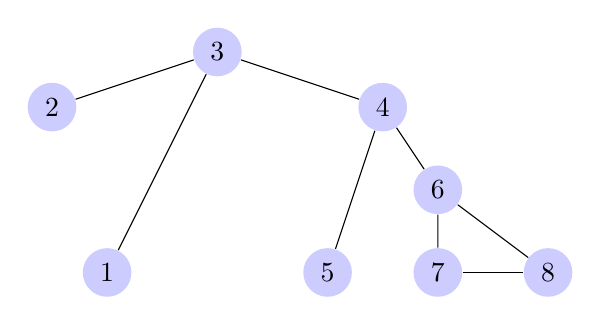
\begin{tikzpicture}
		[scale=.35,auto=left,every node/.style={circle,fill=blue!20}]
		\node (n1) at (0,0) {1};
		\node (n2) at (-2,6)  {2};
		\node (n3)  at (4,8) {3};
		\node (n4) at (10,6)  {4};
		\node (n5) at (8,0)  {5};
		\node (n6) at (12,3)  {6};
		\node (n7) at (12,0)  {7};
		\node (n8) at (16,0)  {8};
		
		\foreach \from/\to in 
		{n5/n4, n2/n3,  n3/n1, n3/n4, n6/n4, n6/n7,n7/n8, n8/n6}
		\draw (\from) -- (\to);
		\end{tikzpicture}
		\caption{$G$ DFS\_Start}
		\label{fig:DFS1}
	\end{figure}
\\
Let's begin a DFS from $v_3$. At the first step we have visited $v_3$ as the starting node, so we look at the nodes which are adjacent to it which are $v_1$, $v_2$, $v_4$:\\
\\
	\begin{figure}[h!]
	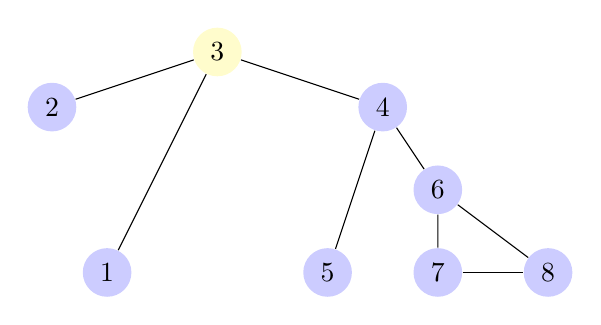
\begin{tikzpicture}
	[scale=.35,auto=left,every node/.style={circle,fill=blue!20}]
	\node (n1) at (0,0) {1};
	\node (n2) at (-2,6)  {2};
	\node[style={circle,fill=yellow!20}] (n3)  at (4,8) {3};
	\node (n4) at (10,6)  {4};
	\node (n5) at (8,0)  {5};
	\node (n6) at (12,3)  {6};
	\node (n7) at (12,0)  {7};
	\node (n8) at (16,0)  {8};
	
	\foreach \from/\to in 
	{n5/n4, n2/n3,  n3/n1, n3/n4, n6/n4, n6/n7,n7/n8, n8/n6}
	\draw (\from) -- (\to);
	\end{tikzpicture}
	\caption{$G$ DFS1}
	\label{fig:DFS1}
\end{figure}

\noindent Following the convention, we visit, $v_1$ due to the lexigraphical ordering, and because we have not yet visited $v_1$. At this point, we look at the neighbouring vertices and notice that the only other vertex is $v_3$ which we have visited. Hence we return to $v_3$'s neighbours in the stack.:\\
\\
\begin{figure}[h!]
	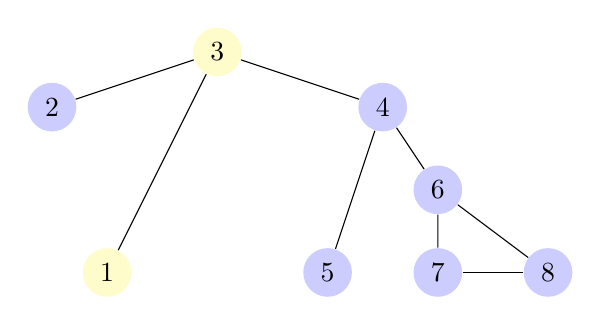
\begin{tikzpicture}
	[scale=.35,auto=left,every node/.style={circle,fill=blue!20}]
	\node[style={circle,fill=yellow!20}] (n1) at (0,0) {1};
	\node (n2) at (-2,6)  {2};
	\node[style={circle,fill=yellow!20}] (n3)  at (4,8) {3};
	\node (n4) at (10,6)  {4};
	\node (n5) at (8,0)  {5};
	\node (n6) at (12,3)  {6};
	\node (n7) at (12,0)  {7};
	\node (n8) at (16,0)  {8};
	
	\foreach \from/\to in 
	{n5/n4, n2/n3,  n3/n1, n3/n4, n6/n4, n6/n7,n7/n8, n8/n6}
	\draw (\from) -- (\to);
	\end{tikzpicture}
	\caption{$G$ DFS2}
	\label{fig:DFS2}
\end{figure}

\noindent Now that we are back at $v_3$'s neighbours in the stack, we visit $v_2$ as this is the next node which has not been visited. Similar to $v_1$, at this point we identify that $v_2$'s only neighbour is $v_3$ which has been visited, and hence $v_2$ is removed from the stack:\\
\\
\begin{figure}[h!]
	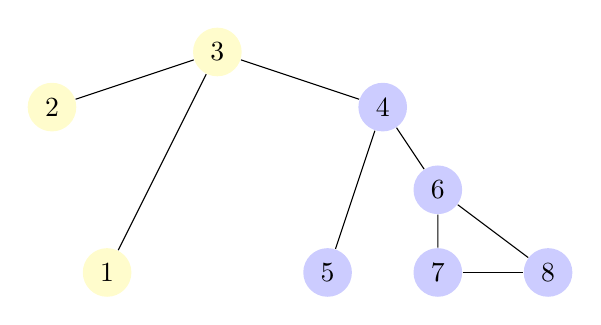
\begin{tikzpicture}
	[scale=.35,auto=left,every node/.style={circle,fill=blue!20}]
	\node[style={circle,fill=yellow!20}] (n1) at (0,0) {1};
	\node[style={circle,fill=yellow!20}]  (n2) at (-2,6)  {2};
	\node[style={circle,fill=yellow!20}] (n3)  at (4,8) {3};
	\node (n4) at (10,6)  {4};
	\node (n5) at (8,0)  {5};
	\node (n6) at (12,3)  {6};
	\node (n7) at (12,0)  {7};
	\node (n8) at (16,0)  {8};
	
	\foreach \from/\to in 
	{n5/n4, n2/n3,  n3/n1, n3/n4, n6/n4, n6/n7,n7/n8, n8/n6}
	\draw (\from) -- (\to);
	\end{tikzpicture}
	\caption{$G$ DFS3}
	\label{fig:DFS3}
\end{figure}

\noindent Now that we are back at $v_3$'s neighbours in the stack, we visit $v_4$ as this is the next node which has not been visited.
\\
\begin{figure}[h!]
	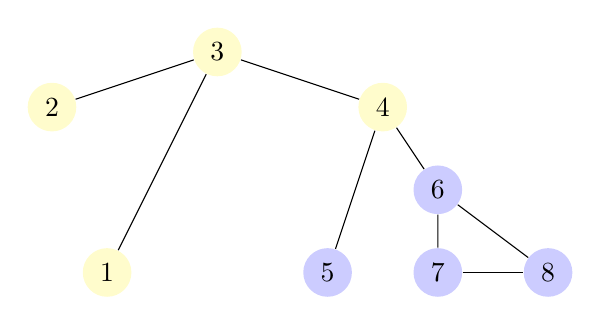
\begin{tikzpicture}
	[scale=.35,auto=left,every node/.style={circle,fill=blue!20}]
	\node[style={circle,fill=yellow!20}] (n1) at (0,0) {1};
	\node[style={circle,fill=yellow!20}]  (n2) at (-2,6)  {2};
	\node[style={circle,fill=yellow!20}] (n3)  at (4,8) {3};
	\node[style={circle,fill=yellow!20}] (n4) at (10,6)  {4};
	\node (n5) at (8,0)  {5};
	\node (n6) at (12,3)  {6};
	\node (n7) at (12,0)  {7};
	\node (n8) at (16,0)  {8};
	
	\foreach \from/\to in 
	{n5/n4, n2/n3,  n3/n1, n3/n4, n6/n4, n6/n7,n7/n8, n8/n6}
	\draw (\from) -- (\to);
	\end{tikzpicture}
	\caption{$G$ DFS4}
	\label{fig:DFS4}
\end{figure}

\noindent Now that we are at $v_4$, we see that $v_4$'s neighbours are $v_5,v_6,v_7$. Hence we look at the vertex with the lowest ordering which is $v_5$ and visit that node.
\\
\begin{figure}[h!]
	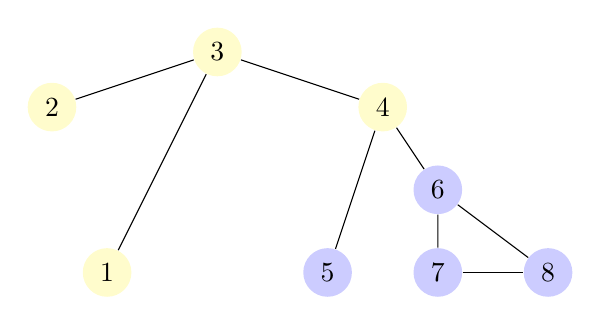
\begin{tikzpicture}
	[scale=.35,auto=left,every node/.style={circle,fill=blue!20}]
	\node[style={circle,fill=yellow!20}] (n1) at (0,0) {1};
	\node[style={circle,fill=yellow!20}]  (n2) at (-2,6)  {2};
	\node[style={circle,fill=yellow!20}] (n3)  at (4,8) {3};
	\node[style={circle,fill=yellow!20}] (n4) at (10,6)  {4};
	\node (n5) at (8,0)  {5};
	\node (n6) at (12,3)  {6};
	\node (n7) at (12,0)  {7};
	\node (n8) at (16,0)  {8};
	
	\foreach \from/\to in 
	{n5/n4, n2/n3,  n3/n1, n3/n4, n6/n4, n6/n7,n7/n8, n8/n6}
	\draw (\from) -- (\to);
	\end{tikzpicture}
	\caption{$G$ DFS5}
	\label{fig:DFS5}
\end{figure}

\noindent Now that we are at $v_5$, we look at the neighbours of $v_5$ but observe that the only neighbour is $v_4$ which has been visited. Hence $v_5$ is removed from the stack and we return to $v_4$.
\\
\begin{figure}[h!]
	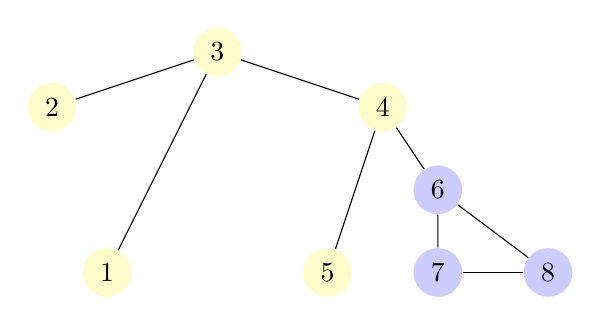
\begin{tikzpicture}
	[scale=.35,auto=left,every node/.style={circle,fill=blue!20}]
	\node[style={circle,fill=yellow!20}] (n1) at (0,0) {1};
	\node[style={circle,fill=yellow!20}]  (n2) at (-2,6)  {2};
	\node[style={circle,fill=yellow!20}] (n3)  at (4,8) {3};
	\node[style={circle,fill=yellow!20}] (n4) at (10,6)  {4};
	\node[style={circle,fill=yellow!20}] (n5) at (8,0)  {5};
	\node (n6) at (12,3)  {6};
	\node (n7) at (12,0)  {7};
	\node (n8) at (16,0)  {8};
	
	\foreach \from/\to in 
	{n5/n4, n2/n3,  n3/n1, n3/n4, n6/n4, n6/n7,n7/n8, n8/n6}
	\draw (\from) -- (\to);
	\end{tikzpicture}
	\caption{$G$ DFS6}
	\label{fig:DFS6}
\end{figure}


\noindent Now that we are at $v_4$ again, we look at the neighbours of $v_4$ and see $v_5$ has been visited so we visit $v_6$.
\\
\begin{figure}[h!]
	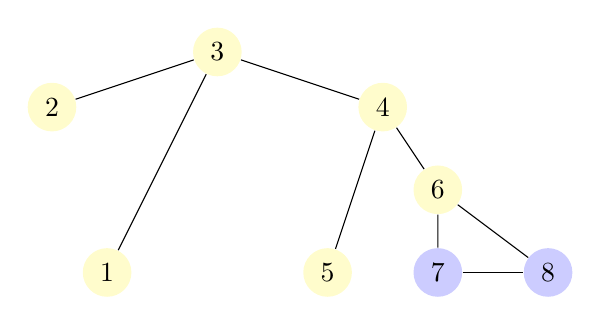
\begin{tikzpicture}
	[scale=.35,auto=left,every node/.style={circle,fill=blue!20}]
	\node[style={circle,fill=yellow!20}] (n1) at (0,0) {1};
	\node[style={circle,fill=yellow!20}]  (n2) at (-2,6)  {2};
	\node[style={circle,fill=yellow!20}] (n3)  at (4,8) {3};
	\node[style={circle,fill=yellow!20}] (n4) at (10,6)  {4};
	\node[style={circle,fill=yellow!20}] (n5) at (8,0)  {5};
	\node[style={circle,fill=yellow!20}] (n6) at (12,3)  {6};
	\node (n7) at (12,0)  {7};
	\node (n8) at (16,0)  {8};
	
	\foreach \from/\to in 
	{n5/n4, n2/n3,  n3/n1, n3/n4, n6/n4, n6/n7,n7/n8, n8/n6}
	\draw (\from) -- (\to);
	\end{tikzpicture}
	\caption{$G$ DFS7}
	\label{fig:DFS7}
\end{figure}
\noindent Now that we are at $v_6$ we look at the neighbours of $v_6$ and see it's neighbours are $v_4$ which is visited, $v_7$, and $v_8$. Following the lexicographical order, we visit $v_7$\\
\begin{figure}[h!]
	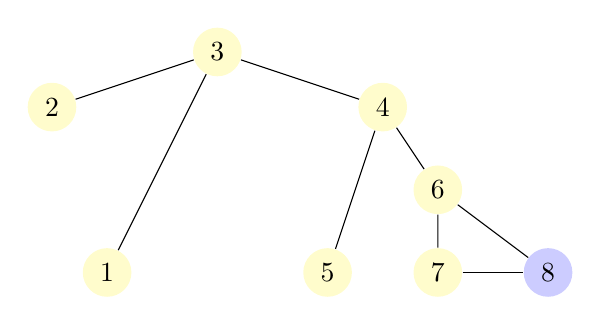
\begin{tikzpicture}
	[scale=.35,auto=left,every node/.style={circle,fill=blue!20}]
	\node[style={circle,fill=yellow!20}] (n1) at (0,0) {1};
	\node[style={circle,fill=yellow!20}]  (n2) at (-2,6)  {2};
	\node[style={circle,fill=yellow!20}] (n3)  at (4,8) {3};
	\node[style={circle,fill=yellow!20}] (n4) at (10,6)  {4};
	\node[style={circle,fill=yellow!20}] (n5) at (8,0)  {5};
	\node[style={circle,fill=yellow!20}] (n6) at (12,3)  {6};
	\node[style={circle,fill=yellow!20}] (n7) at (12,0)  {7};
	\node (n8) at (16,0)  {8};
	
	\foreach \from/\to in 
	{n5/n4, n2/n3,  n3/n1, n3/n4, n6/n4, n6/n7,n7/n8, n8/n6}
	\draw (\from) -- (\to);
	\end{tikzpicture}
	\caption{$G$ DFS8}
	\label{fig:DFS8}
\end{figure}
\\
\\
\noindent Now that we are at $v_7$ we look at the neighbours of $v_7$ and see it's neighbours are $v_4$ which is visited, $v_6$ which is visited, and $v_8$. Next we visit $v_8$
\\
\begin{figure}[h!]
	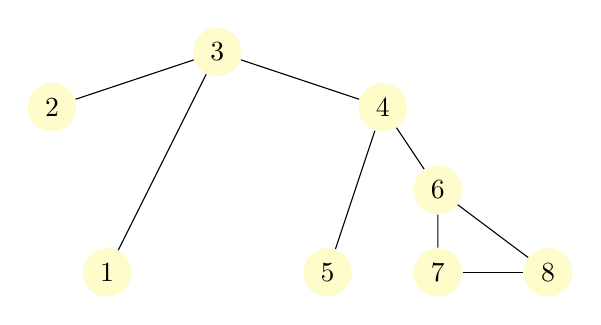
\begin{tikzpicture}
	[scale=.35,auto=left,every node/.style={circle,fill=blue!20}]
	\node[style={circle,fill=yellow!20}] (n1) at (0,0) {1};
	\node[style={circle,fill=yellow!20}]  (n2) at (-2,6)  {2};
	\node[style={circle,fill=yellow!20}] (n3)  at (4,8) {3};
	\node[style={circle,fill=yellow!20}] (n4) at (10,6)  {4};
	\node[style={circle,fill=yellow!20}] (n5) at (8,0)  {5};
	\node[style={circle,fill=yellow!20}] (n6) at (12,3)  {6};
	\node[style={circle,fill=yellow!20}] (n7) at (12,0)  {7};
	\node[style={circle,fill=yellow!20}] (n8) at (16,0)  {8};
	
	\foreach \from/\to in 
	{n5/n4, n2/n3,  n3/n1, n3/n4, n6/n4, n6/n7,n7/n8, n8/n6}
	\draw (\from) -- (\to);
	\end{tikzpicture}
	\caption{$G$ DFS9}
	\label{fig:DFS9}
\end{figure}
\\
\noindent At this stage, we are at $v_8$ and have visited every node. Hence each vertex is removed from the stack and we conclude the example.
\end{example}


\begin{figure}[h!]
	\centering
	\includegraphics[width=1\linewidth]{bfs}
	\caption{BFS Algorithm from Lecture 16}
	\label{fig:BFS}
\end{figure}
In the breadth first search algorithm, rather than following one path continuously to traverse the graph, we visit all neighbouring nodes simultaneously. When we want to visit one particular instance and determine all possible outcomes or neighbours, using DFS 


\begin{example}
	As in our previous example, consider the graph:\\
	\begin{figure}[h!]
		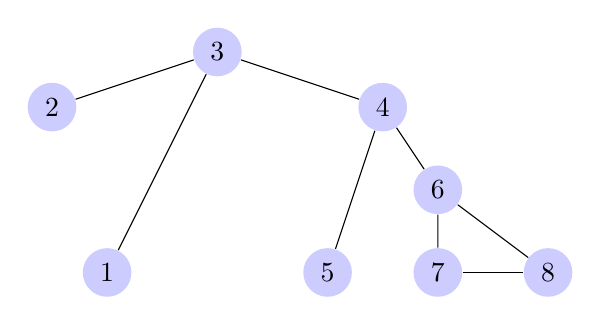
\begin{tikzpicture}
		[scale=.35,auto=left,every node/.style={circle,fill=blue!20}]
		\node (n1) at (0,0) {1};
		\node (n2) at (-2,6)  {2};
		\node (n3)  at (4,8) {3};
		\node (n4) at (10,6)  {4};
		\node (n5) at (8,0)  {5};
		\node (n6) at (12,3)  {6};
		\node (n7) at (12,0)  {7};
		\node (n8) at (16,0)  {8};
		
		\foreach \from/\to in 
		{n5/n4, n2/n3,  n3/n1, n3/n4, n6/n4, n6/n7,n7/n8, n8/n6}
		\draw (\from) -- (\to);
		\end{tikzpicture}
		\caption{$G$ BFS\_Start}
		\label{fig:DFS1}
	\end{figure}
We will conduct a BFS on this algorithm, stating at node $v_3$.\\
\\
At the first step we have visited $v_3$ as the starting node, so we look at the nodes which are adjacent to it which are $v_1$, $v_2$, $v_4$:\\
\\
\begin{figure}[h!]
	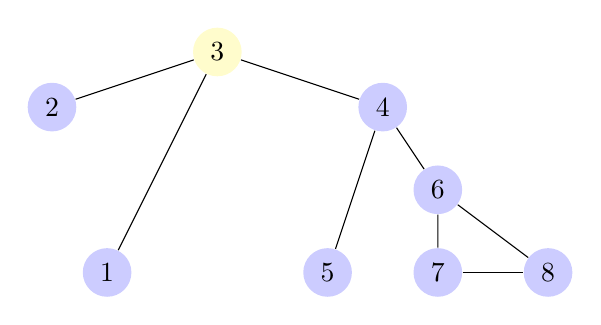
\begin{tikzpicture}
	[scale=.35,auto=left,every node/.style={circle,fill=blue!20}]
	\node (n1) at (0,0) {1};
	\node (n2) at (-2,6)  {2};
	\node[style={circle,fill=yellow!20}] (n3)  at (4,8) {3};
	\node (n4) at (10,6)  {4};
	\node (n5) at (8,0)  {5};
	\node (n6) at (12,3)  {6};
	\node (n7) at (12,0)  {7};
	\node (n8) at (16,0)  {8};
	
	\foreach \from/\to in 
	{n5/n4, n2/n3,  n3/n1, n3/n4, n6/n4, n6/n7,n7/n8, n8/n6}
	\draw (\from) -- (\to);
	\end{tikzpicture}
	\caption{$G$ BFS1}
	\label{fig:BFS1}
\end{figure}
\\
\noindent We visit each of the neighbours of $v_3$.\\
\\
\begin{figure}[h!]
	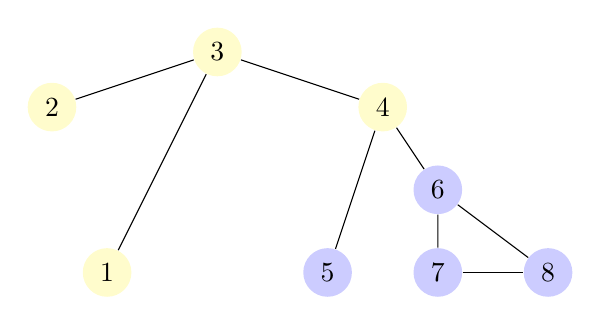
\begin{tikzpicture}
	[scale=.35,auto=left,every node/.style={circle,fill=blue!20}]
	\node[style={circle,fill=yellow!20}] (n1) at (0,0) {1};
	\node[style={circle,fill=yellow!20}] (n2) at (-2,6)  {2};
	\node[style={circle,fill=yellow!20}] (n3)  at (4,8) {3};
	\node[style={circle,fill=yellow!20}] (n4) at (10,6)  {4};
	\node (n5) at (8,0)  {5};
	\node (n6) at (12,3)  {6};
	\node (n7) at (12,0)  {7};
	\node (n8) at (16,0)  {8};
	
	\foreach \from/\to in 
	{n5/n4, n2/n3,  n3/n1, n3/n4, n6/n4, n6/n7,n7/n8, n8/n6}
	\draw (\from) -- (\to);
	\end{tikzpicture}
	\caption{$G$ BFS2}
	\label{fig:BFS2}
\end{figure}

\noindent We examine $v_1$, $v_2$, and $v_4$ We see that $v_2$ and $v_1$ only have $v_3$ as a neighbour which is visited, while $v_4$ has neighbours $v_5$ and $v_6$, so we visit these\\
\\
\begin{figure}[h!]
	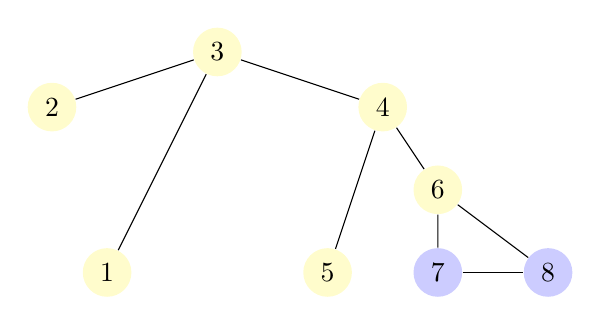
\begin{tikzpicture}
	[scale=.35,auto=left,every node/.style={circle,fill=blue!20}]
	\node[style={circle,fill=yellow!20}] (n1) at (0,0) {1};
	\node[style={circle,fill=yellow!20}] (n2) at (-2,6)  {2};
	\node[style={circle,fill=yellow!20}] (n3)  at (4,8) {3};
	\node[style={circle,fill=yellow!20}] (n4) at (10,6)  {4};
	\node[style={circle,fill=yellow!20}]  (n5) at (8,0)  {5};
	\node[style={circle,fill=yellow!20}]  (n6) at (12,3)  {6};
	\node (n7) at (12,0)  {7};
	\node (n8) at (16,0)  {8};
	
	\foreach \from/\to in 
	{n5/n4, n2/n3,  n3/n1, n3/n4, n6/n4, n6/n7,n7/n8, n8/n6}
	\draw (\from) -- (\to);
	\end{tikzpicture}
	\caption{$G$ BFS3}
	\label{fig:BFS3}
\end{figure}

\noindent We examine $v_5$, and $v_6$. We see that $v_5$ only has $v_6$ as a neighbour which is visited, while $v_6$ has neighbours $v_7$ and $v_8$, so we visit these\\
\\
\begin{figure}[h!]
	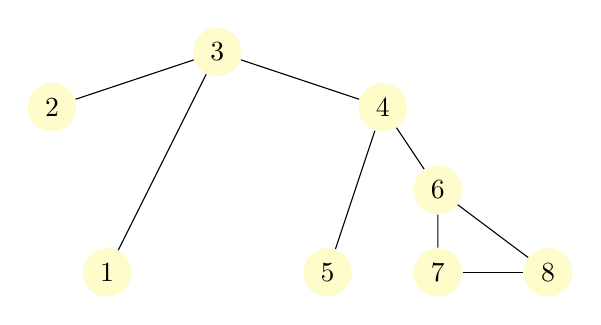
\begin{tikzpicture}
	[scale=.35,auto=left,every node/.style={circle,fill=blue!20}]
	\node[style={circle,fill=yellow!20}] (n1) at (0,0) {1};
	\node[style={circle,fill=yellow!20}] (n2) at (-2,6)  {2};
	\node[style={circle,fill=yellow!20}] (n3)  at (4,8) {3};
	\node[style={circle,fill=yellow!20}] (n4) at (10,6)  {4};
	\node[style={circle,fill=yellow!20}]  (n5) at (8,0)  {5};
	\node[style={circle,fill=yellow!20}]  (n6) at (12,3)  {6};
	\node[style={circle,fill=yellow!20}] (n7) at (12,0)  {7};
	\node[style={circle,fill=yellow!20}] (n8) at (16,0)  {8};
	
	\foreach \from/\to in 
	{n5/n4, n2/n3,  n3/n1, n3/n4, n6/n4, n6/n7,n7/n8, n8/n6}
	\draw (\from) -- (\to);
	\end{tikzpicture}
	\caption{$G$ BFS3}
	\label{fig:BFS3}
\end{figure}

\noindent We examine $v_7$, and $v_8$. We see that all their neighbouring nodes are visited and the process is complete.\\

\end{example}

\section{Conclusion}
\noindent In this paper we have examined the topics covered in lecture 16, most notably examining the graphs and some key definitions surrounding graphs, the history of Graph Theory and some motivating modern examples of graph applications, the Graph ADT with a particular focus on unweighted and undirected graphs, operations on a graph, and the BFS and DFS algorithms. This concludes the topics which were covered in Lecture 16.

\section{Acknowledgements}
\noindent The authors wish to thank MATH20150 for directing the definitions used in section \ref{intro} and notation in section \ref{repr}, and the Tikz package authors for providing the graphing tools to produce the included graphs.

\end{document}

